\chapter{Implementation}
Two components of the system have been implemented as a proof of concept: the editor and the web 3D view.

\paragraph{Editor} The editor has been implemented as a combination of Electron application with Python backend. A portable Python version is a part of the application executable; therefore, it is unnecessary to have Python installed globally. The backend is capable of loading user-defined functions. In order to create a user-defined function:
\begin{enumerate}
    \item create a new \verb|.py| script in the \verb|src/py/scripts| directory,
    \item import the \verb|param| and \verb|output| decorators from the parameters module (this is the only necessary API),
    \item create a function called \verb|call|
\end{enumerate}
The following example illustrates the API available for creating custom functions. All parameters and return values have to be documented by the decorators. The prototype UI is presented in figure \ref{fig:editorDemo}.
\begin{minted}[
    linenos,
    numbersep=5pt,
    gobble=0,
    frame=lines,
    framesep=2mm]{python}
from parameters import param, output

@param('a', 'number') #(first input parameter name, type)
@param('b', 'number') #(second input parameter name, type)
@output('sum', 'number') #(first output parameter name, type)
def call(a, b):
    return a + b
\end{minted}

The build of the application into an executable deployable form is fairly complex:
\begin{enumerate}
    \item package the underlying electron application,
    \item download and inject portable version of Python 3 into the packaged app,
    \item install Python dependencies locally into the portable version,
    \item and package the application into a downloadable archive.
\end{enumerate}
This procedure can be executed on both Linux and Windows, as all of the used technologies are multiplatform. To simplify this process, a Github Action has been set up on github.com. The Action performs all of the steps above once a new version of the source code has been uploaded and tagged for release. The packaged version of the prototype can be downloaded from Github\footnote{See section Releases at \url{https://github.com/vojtatom/urbann}}.

\begin{figure}[h]
    \centering
    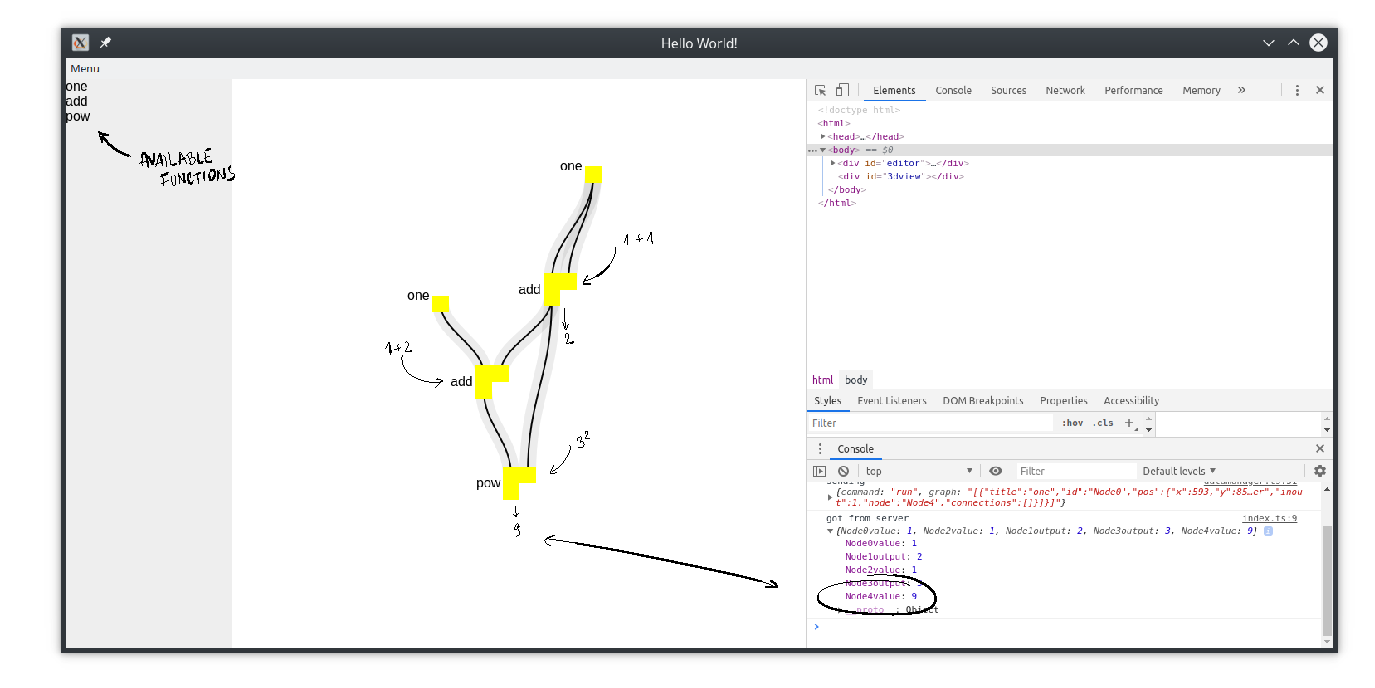
\includegraphics[width=\linewidth]{figures/editorDemo2.pdf}
    \caption{Demonstration of the visual programming pipeline calling Python functions in the background}
    \label{fig:editorDemo}
\end{figure}


\paragraph{Web 3D View}
The Web 3D View renders processed geometry extracted from CityJSON. The displayed area is located in Holešovice, Prague\footnote{The data was provided by courtesy of IPR Prague}. The geometry and metadata have been processed using the following pipeline:
\begin{enumerate}
    \item original CityJSON is converted to \verb|.obj| using \cite{cjio},
    \item a set of custom readers\footnote{See \url{https://github.com/vojtatom/citypy}} loads the original CityJSON data together with OBJ of terrain and buildings and pairs the geometry with available metadata,
    \item a heightmap of the roads and terrain is generated,
    \item all generated data (geometry, metadata, and heightmap) are packed into a JSON file,
    \item the file is exported to the web 3D viewer  
\end{enumerate}
The code of the web 3D view is also available on Github\footnote{See \url{https://github.com/vojtatom/metacity}}. The web view is implemented using pure WebGL 2; it loads the geometry structured as outlined in the previous chapter, see section \ref{sec:inputrepres}. For illustration, there is a live demo available online\footnote{See \url{https://vojtatom.cz/metacity}}, or see figures \ref{fig:metacit1}-- \ref{fig:metacit5}.


\begin{figure}[h]
    \centering
    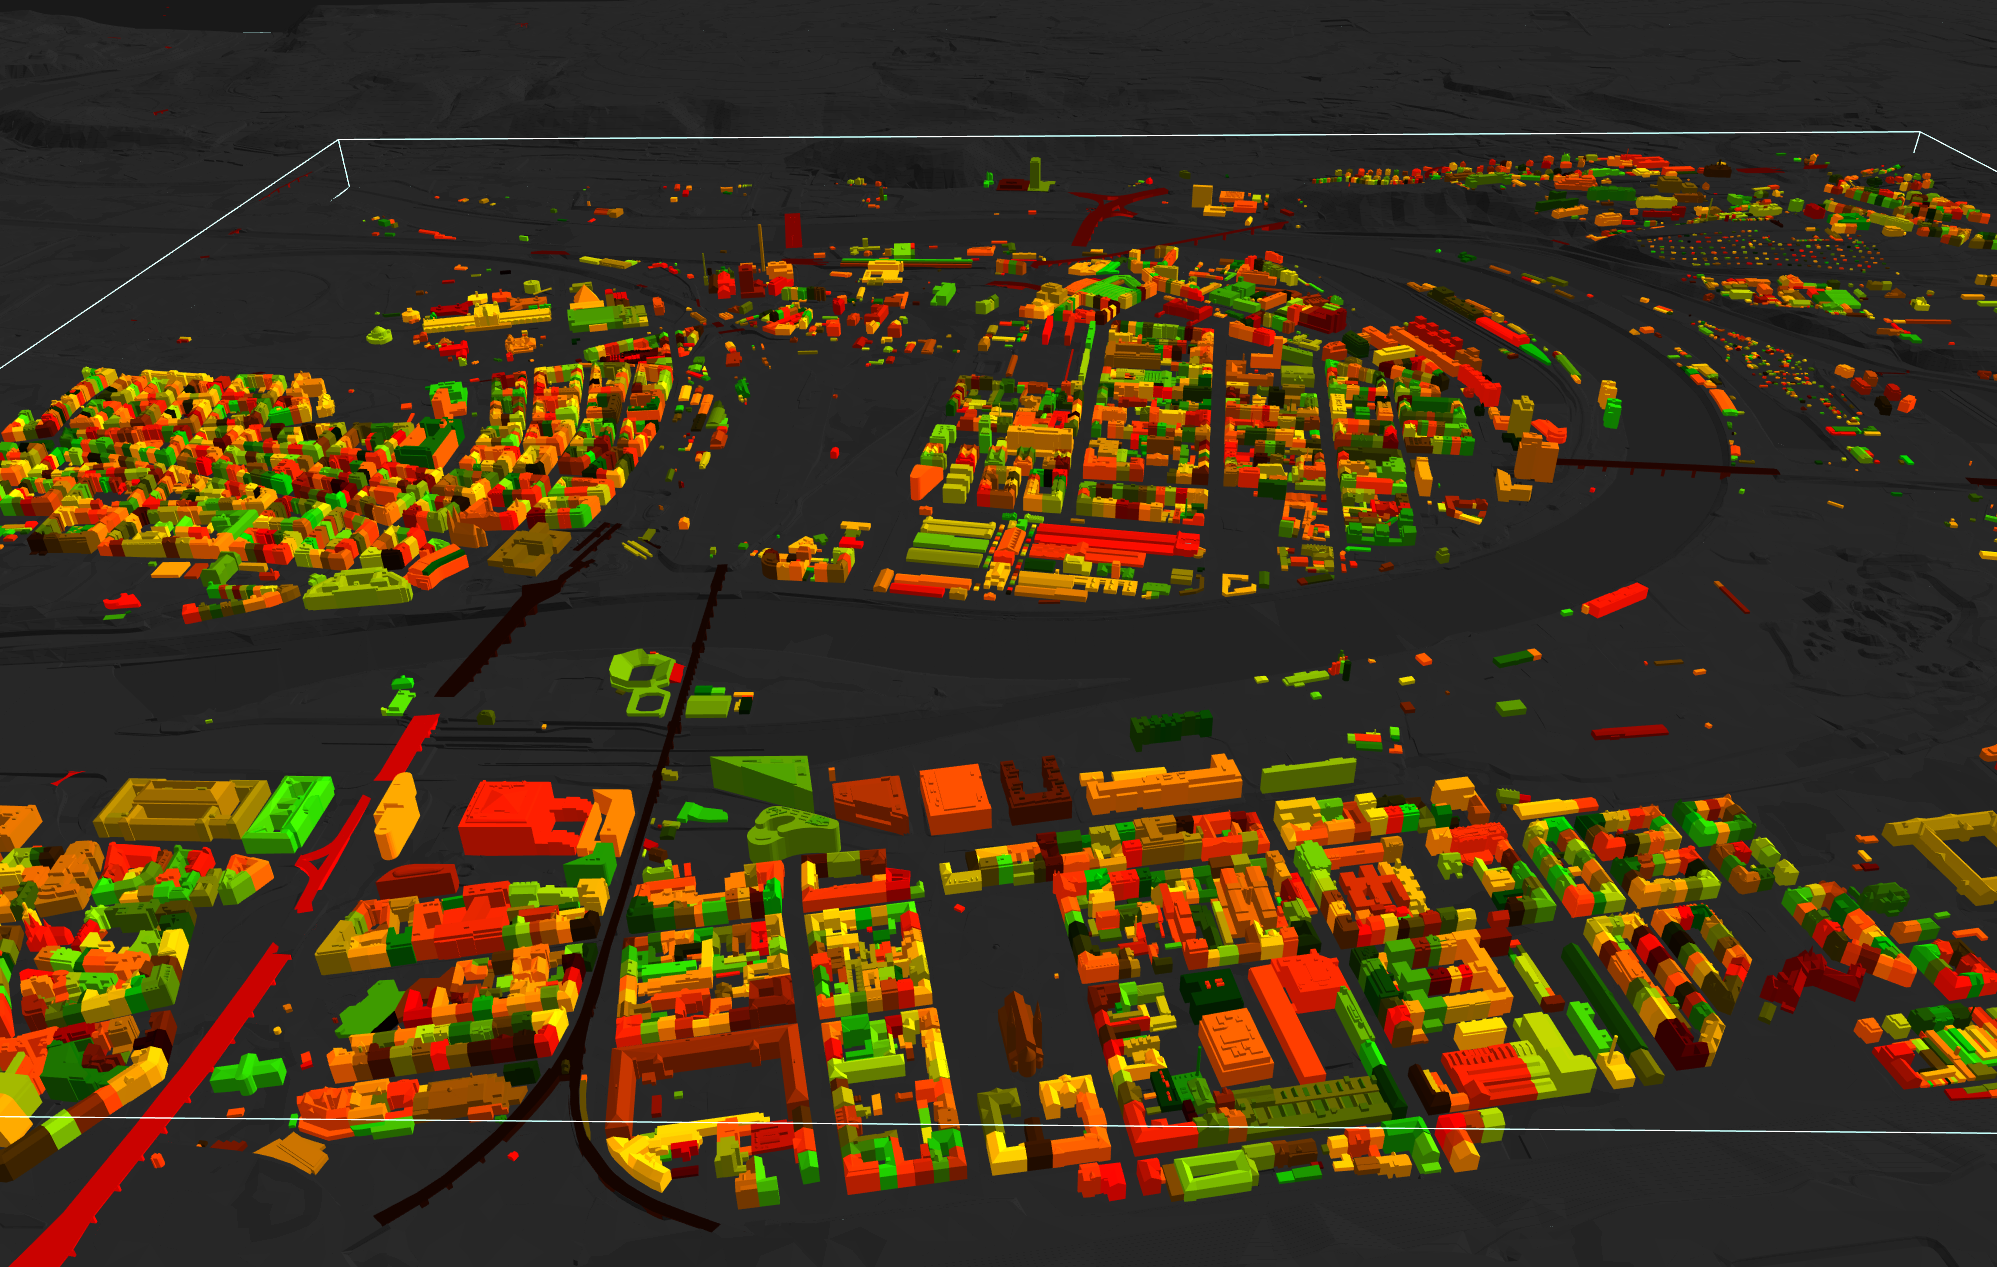
\includegraphics[width=\linewidth]{figures/metacity0.png}
    \caption{Loading terrain and building geometry, side view}
    \label{fig:metacit1}
\end{figure}

\begin{figure}[h]
    \centering
    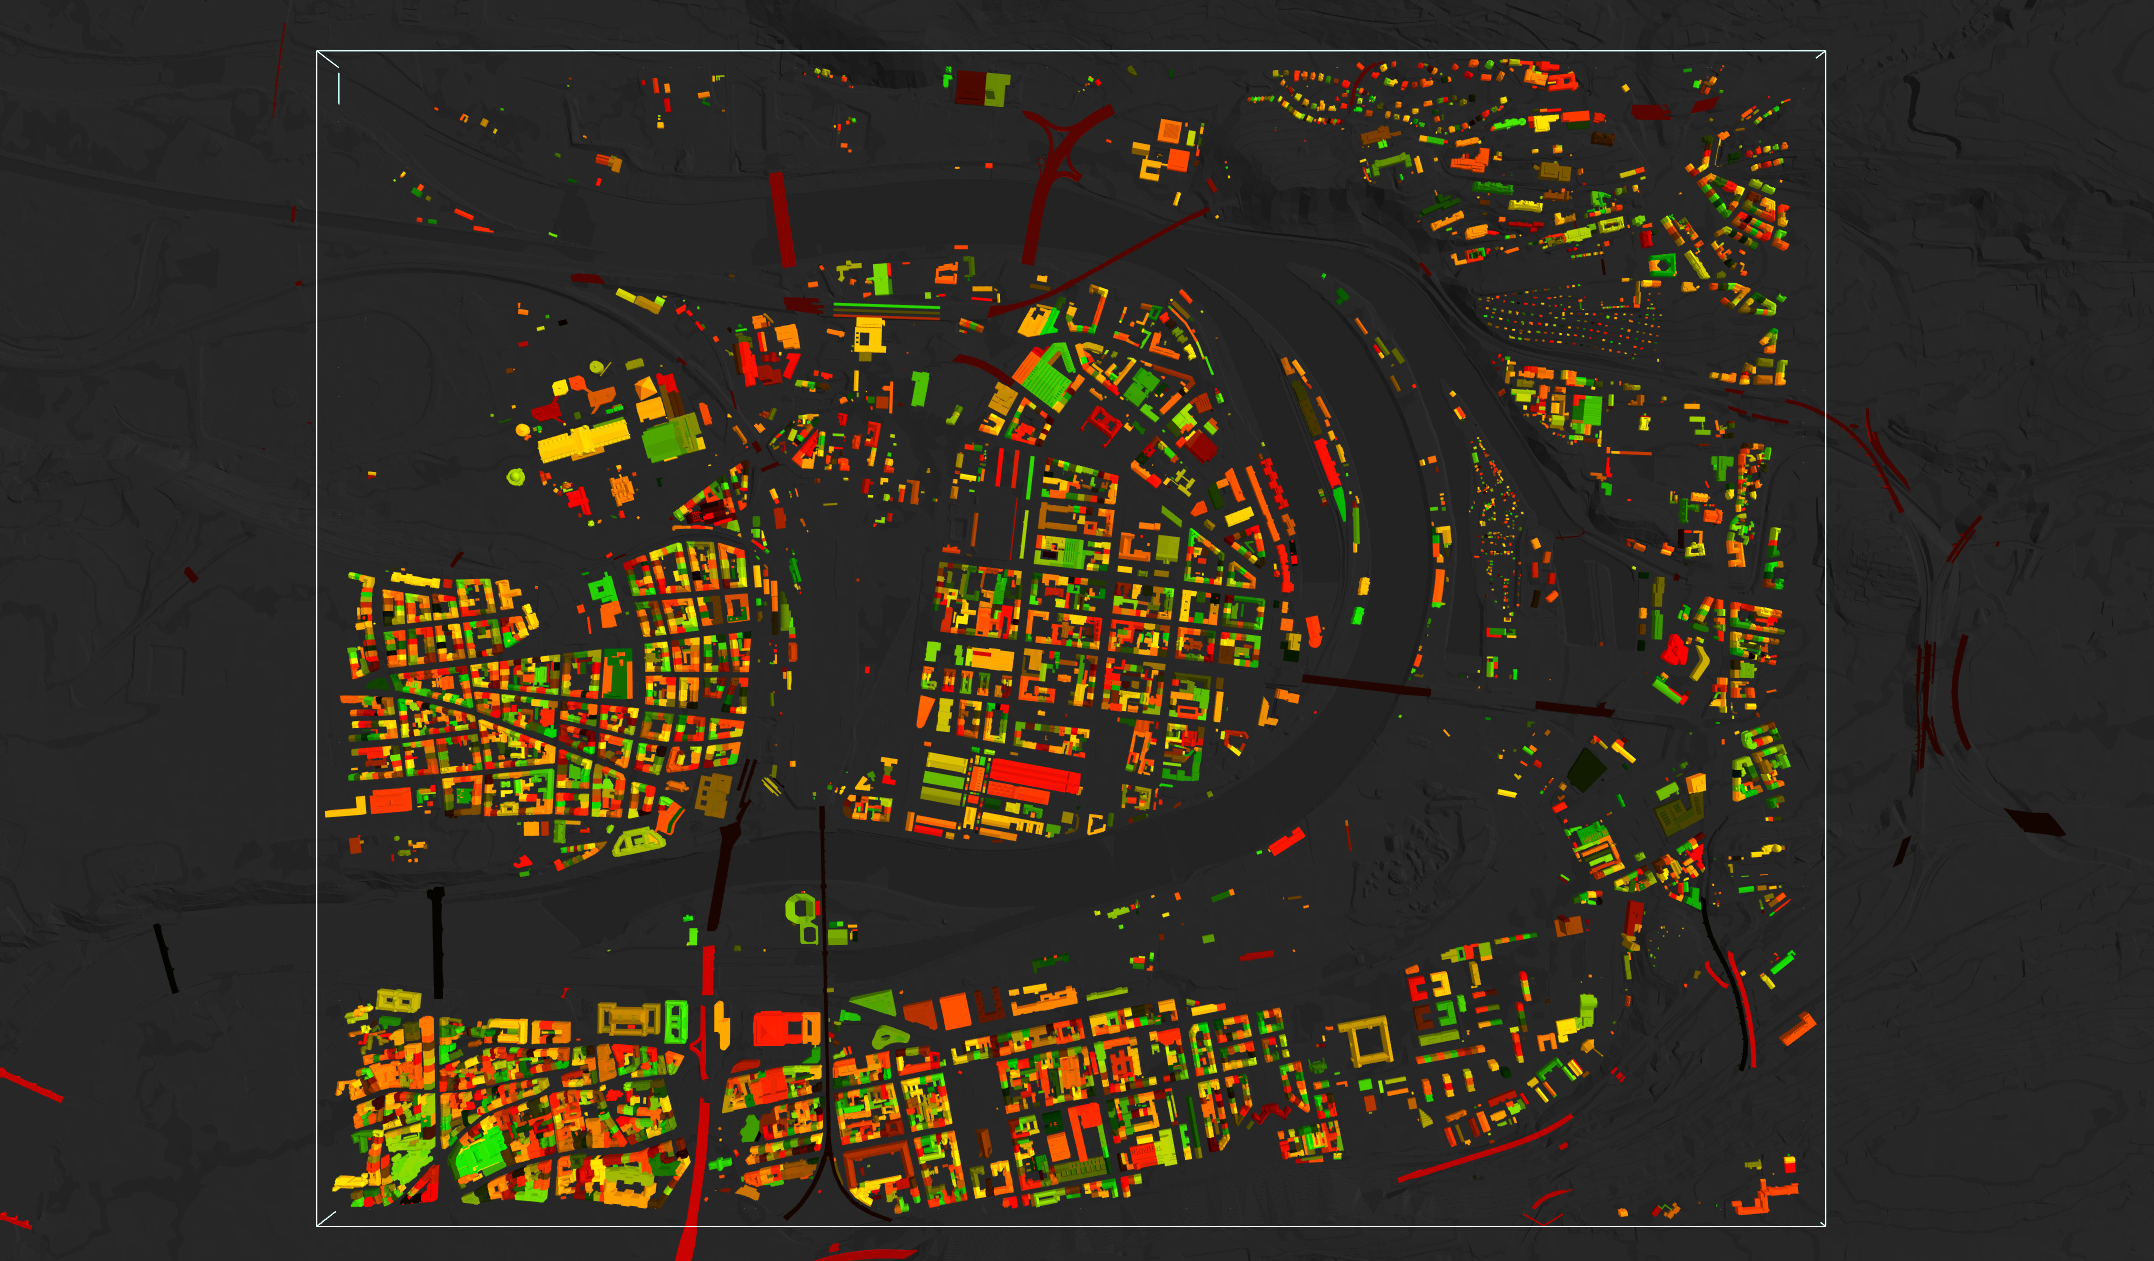
\includegraphics[width=\linewidth]{figures/webPrototype1.png}
    \caption{Loading terrain and building geometry, top view}
\end{figure}

\begin{figure}[h]
    \centering
    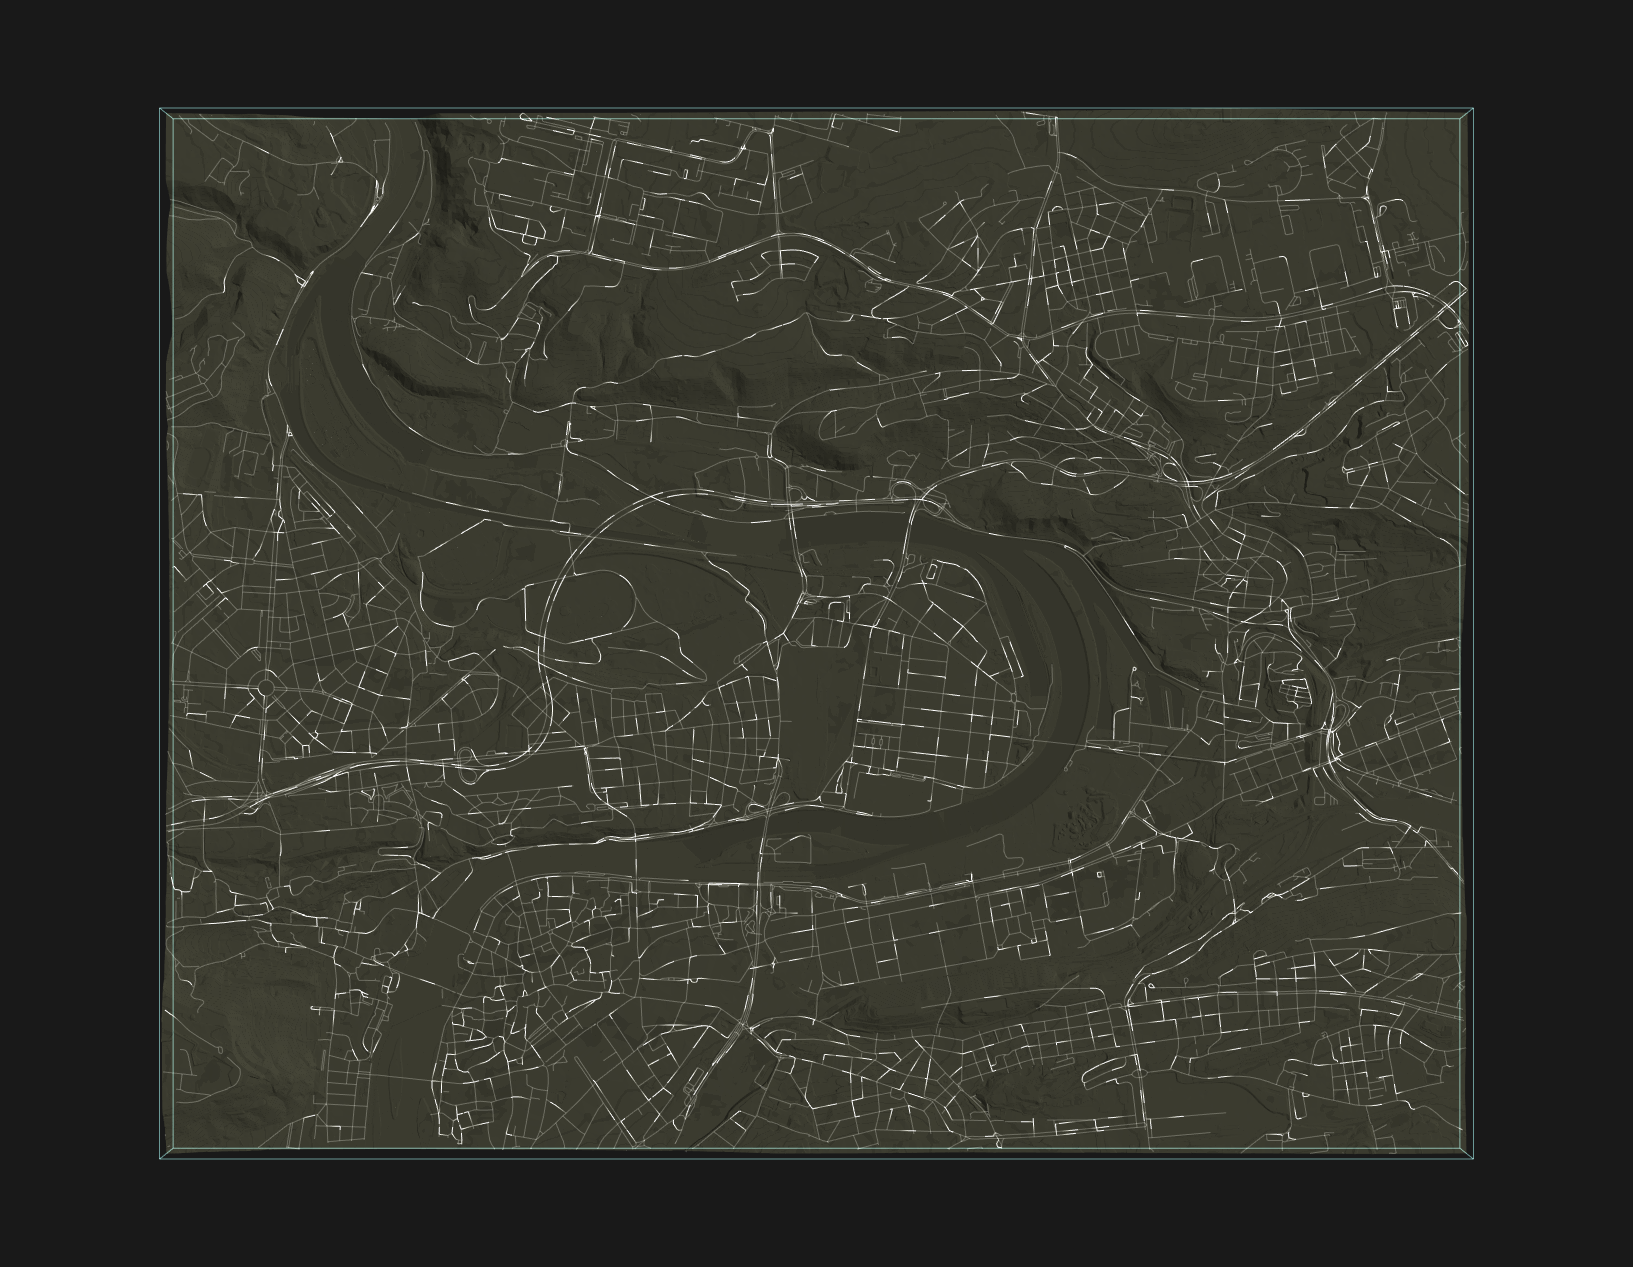
\includegraphics[width=\linewidth]{figures/webPrototype2.png}
    \caption{Prototyping animated traffic}
\end{figure}

\begin{figure}[h]
    \centering
    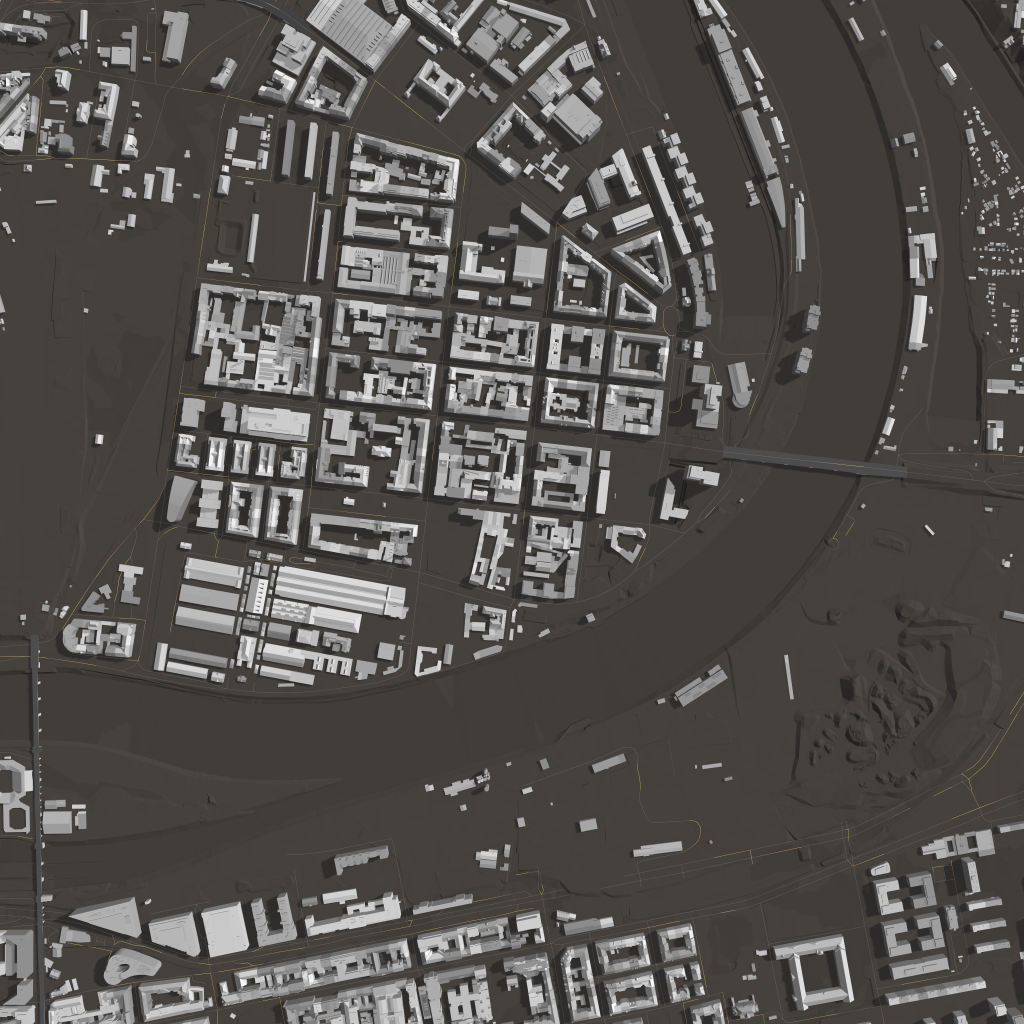
\includegraphics[width=\linewidth]{figures/metacity2.png}
    \caption{Implementing building shadows, top view}
\end{figure}

\begin{figure}[h]
    \centering
    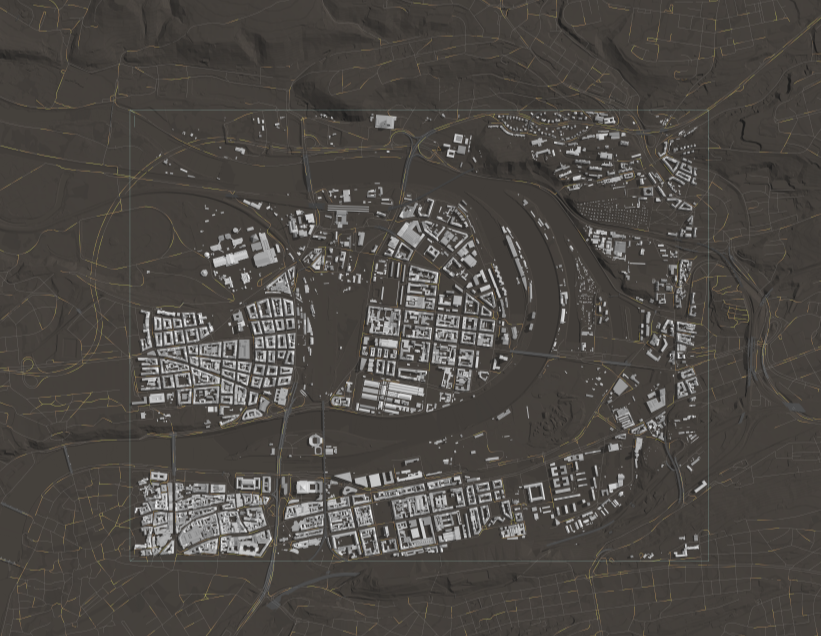
\includegraphics[width=\linewidth]{figures/metacity3.png}
    \caption{Implementing building shadows, side view}
    \label{fig:metacit5}
\end{figure}

\section{Future Development}
Some research and implementation areas have not been explored yet. These topics will be the focus of future development:
\begin{itemize}
    \item generating outputs for physical models production and assembly,
    \item projection mapping the visualization onto a physical model,
    \item defining the basic styling functionalities,
    \item user testing the editor interface,
    \item and combining all component prototypes.
\end{itemize}


\chapter{Conclusion}
The report described and analyzed urban data --- the sources, domains, and used file formats. Urban data alone is not always sufficient to generate the insight; analytical models derived from the data together with interactive tools can improve the city planning process. The initial research presented a number of existing visualization tools. Some of these tools are purely virtual; others are augmented by the use of physical components.
With the three main goals in mind, the design of a modular visualization system was presented. The proposed design uses a combination of different technologies to provide a combination of flexibility, customizability, and high performance. Two prototypes of system components have been implemented. The two protoypes presented in this report demonstrated that the design concepts introduced in the previous chapter are plausible. The future development will include the integration of individual components into a functional standalone application. 
